
\documentclass[10pt]{article}
\usepackage[utf8]{inputenc}
\usepackage{kotex}
\usepackage{graphicx}
\usepackage{subfigure}
\usepackage{titling}
\setlength{\droptitle}{-2cm}
\usepackage{array}
\usepackage{amssymb}
\usepackage{amsmath}
\usepackage{siunitx} 
\usepackage{enumerate} 
\usepackage{pgfplots}
\usepackage{pgfplotstable}
\usepackage{tikz,pgfplots}
\usepackage{wasysym}
\usepackage{geometry}
\usepackage{authblk}
\usepackage{kotex}
\usepackage{bibunits}
\usepackage{tabularx}
\usepackage{hyperref}
\usepackage{pythonhighlight}
\usepackage[toc,page]{appendix}


\geometry{
    a4paper,
    total={170mm,257mm},
    left=20mm,
    top=20mm,
}

\title{\textbf{Mathematical Foundation of DNN : HW 2}}
\author{Jeong Min Lee}

\begin{document}
\maketitle
In this assigment, I implemented every algorithms both with torch package and without it(except problem 7). 
I'll focus on the result of optimization and the comparison to both implmentations. Also, I attached the code what I used in this assignment in appendix of this document. Please refer to it if you need.
\section*{1}

I refer the code given by lecture to implement the SGD with logistic regression. The result of this code is 
described in figure \ref{fig1}. As figure \ref{fig1} depicted, both implementation succeeded convergence, since their losses were decreasing and saturated.
Since the algorithm without torch and optimizer is too naive, the performace of SGD without torch is worse than that with torch. To be specific, 
the result drawn by SGD without torch has large variance. I guess the optimizer torch using is more sophisticated and effective. This tendency kept appearing the following problems.

\begin{figure}[!h]
    \begin{center}
        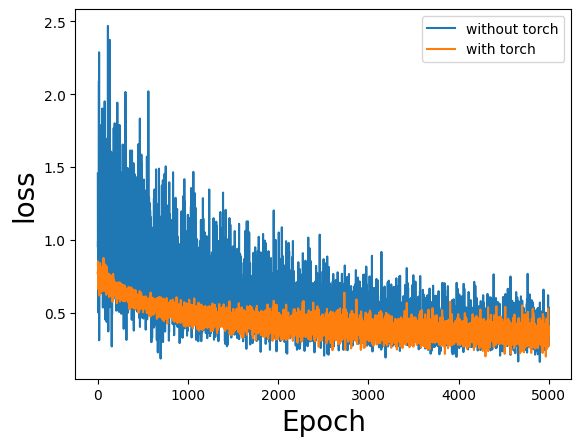
\includegraphics[scale = 0.5]{../hw2/fig/prob1.png}
        \label{fig1}
    \end{center}
    \caption{The comparison of the algorithm of SGD both with torch and without it.}
\end{figure}

\section*{2}
Simiar to problem 1, both algorithm were successful to converge. In this problem, both implementation success to converge like logistic regression.
It is noteworthy that the implementation without torch is unstable about 200 epochs rather than the one with torch. 
Furthermore,I compared the performance of SVM optimization and logistic regression. As figure \ref{fig2} (b) depicted, the optimization with SVM is better than logistic regression with respect to its faster convergence and stability.
% In this problem, my own SGD algorithm converged but not to zero, unlike the other optimization algorithms.
% I made several assumptions about the reason of poorness of SVM implementation without torch package
% First of all, I think this issue came from the non-differentiability of ReLU function and lack of the exception controll on my algorithm.
% However, when I counted the number of hit that SGD meet the non-differential point within its training, it result in zero, that is, SGD never meet non-differentiable point in its training process. 
% Next,I conjecture that this is from the issue of hyperparameter tuning and initialization. 
% The only one that I can revise among the given hyperparameters is learning rate.
% I've tried almost 20 distinct learning rate but they are not satisfactory.
% Finally, I'm convinced that this may related with the gradient update.
% When I print the norm of model weight, my own alrogithm has approximately 10 times larger weight. 
% Since I implement SGD with batch size 8, the reasonable gradient update of each batch would be the average of gradient accumulated while iterating the batch.
% Again, this cannot attain the level of optimization with torch. I've tried the random selection among the gathered gradient, which results in similar performance to prior one. 

\begin{figure}[!h]
    \begin{center}
        \subfigure[]{
            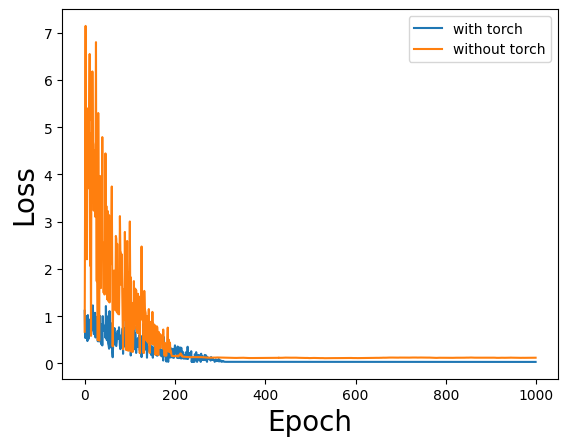
\includegraphics[scale = 0.5]{../hw2/fig/prob2.png}
        }
        \subfigure[]{
            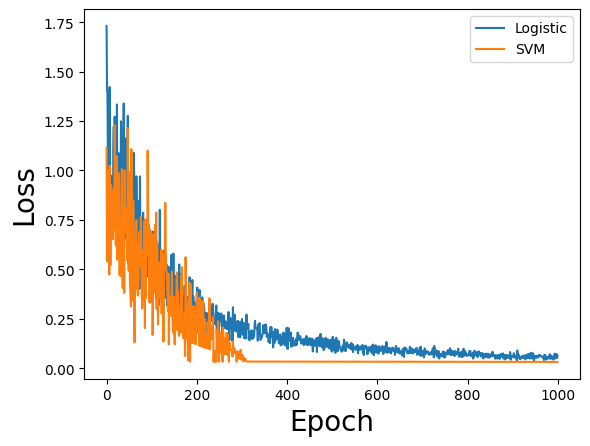
\includegraphics[scale = 0.5]{../hw2/fig/prob2_2.png}
        }
        \label{fig2}
    \end{center}
    \caption{(a) The comparison of the algorithm of SGD both with torch and without it. (b) The comparision between logistic regression and SVM. I used the algorithm without the torch.}
\end{figure}


\section*{3}

As one can check from figure \ref{fig3}, the given data is not linearly separable, that is, there is no line that separate both red and blue dot into two sectors.
However, after transform the $X$ using $\varphi$, this data can be linearly separable. To calculate the decision boundary, I used SVM which is more superior than logistic regression.
Again, I attached the implementation at the appendix. 
\begin{figure}[!h]
    \begin{center}
        \subfigure[]{
            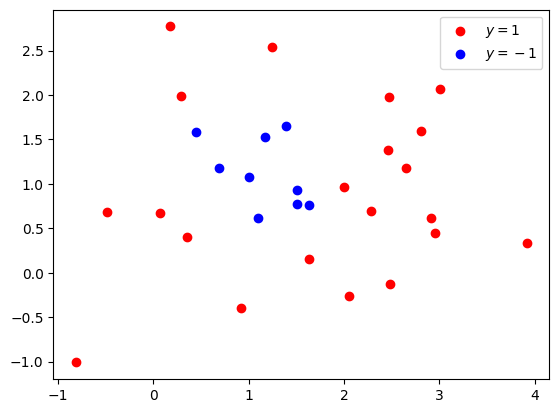
\includegraphics[scale = 0.5]{../hw2/fig/prob3.png}
        }
        \subfigure[]{
            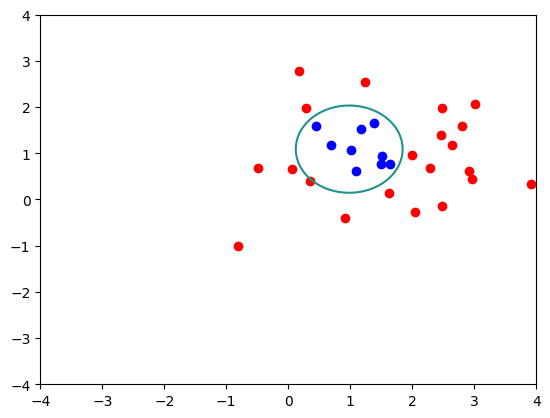
\includegraphics[scale = 0.5]{../hw2/fig/prob3_2.png}
        }
    \end{center}
    \caption{(a) The scatter plot of given data with its label. (b) The scatter plot with decision boundary(green) obtained by SVM.}
    \label{fig3}
\end{figure}

\begin{figure}[!h]
    \begin{center}
        \subfigure{
            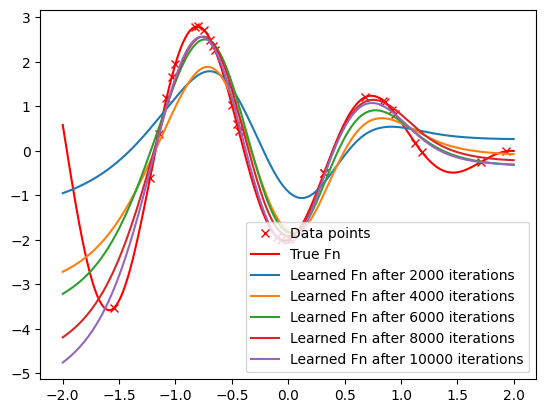
\includegraphics[scale = 0.5]{fig/prob7.png}
        }
        \subfigure{
            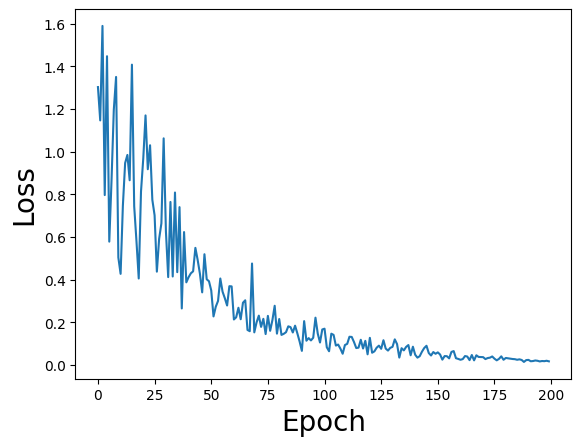
\includegraphics[scale = 0.5]{fig/prob7_2.png}
        }
    \end{center}
    \label{fig4}
    \caption{(a) The result of SGD training. One can notice that as SGD learned more, the $f_\theta$ became more similar to true function. (b) This figure shows that the SGD train was success. }
\end{figure}

\clearpage
\section*{4,5}
I proved problem 4 and 5 at the same time. 
\textbf{CLAIM} : $y = -\log(x)$ function is strict convex function. 
\\To prove the \textbf{CLAIM} above, I proved the following \textbf{LEMMA}.\\
\textbf{LEMMA} : The differentiable function $f$ is strictly convex \textit{if and only if} its derivate $f^\prime$ is strictly increasing.
\textbf{proof}\\
$\implies :     a,b \in \mathbb{R} (a<b). \text{ Let} x_1, x_2, x_3 \in \mathbb{R} \text{ be chosen s.t. } a<x_1<x_2<x_3<b.$

From Chordal Slope Lemma, which is famous lemma applicable to convex function, the following inequalities are held.

\begin{equation}
    \frac{f(x_1) - f(a)}{x_1 - a} < \frac{f(x_2) - f(x_1)}{x_2 - x_1}<\frac{f(x_3) - f(x_2)}{x_3 - x_2} < \frac{f(b) - f(x_3)}{b - x_3}
    \label{eqn1}
\end{equation} 
\begin{equation}
    \frac{f(x_2) - f(a)}{x_2 - a} < \frac{f(b) - f(x_2)}{b - x_2}
\end{equation} 

Taking limit $x_1 \rightarrow a, x_3 \rightarrow b$ on equation \ref{eqn1}, 

\begin{equation}
    f^\prime(a) \le \frac{f(x_2) - f(a)}{x_2 - a} < \frac{f(b) - f(x_2)}{b - x_2} \le f^\prime(b)
\end{equation}\\
and, therefore, $f^\prime(a)<f^\prime(b)$ for arbitrary $a,b\in\mathbb{R}$.\\

$\Longleftarrow$ : Let $x_1, x_2, x_3 \in \mathbb{R}$ s.t. $x_1<x_2<x_3$. From Mean Value Theorem,
\begin{equation}
    \exists a \text{ s.t } \frac{f(x_2) - f(x_1)}{x_2 - x_1} = f^\prime(a) \\
\end{equation}
\begin{equation}
    \exists b \text{ s.t } \frac{f(x_3) - f(x_2)}{x_3 - x_2} = f^\prime(b)
\end{equation}
Note that $x_1<a<x_2<b<x_3$. Since $f^\prime$ is strictly increasing, $f^\prime(a) < f^\prime(b)$, which implies 
\begin{equation}
    \frac{f(x_2) - f(x_1)}{x_2 - x_1} < \frac{f(x_3) - f(x_2)}{x_3 - x_2} 
    \label{eqn6}
\end{equation}
The result of equation \ref{eqn6} is equivalent that $f$ is strictly convex according to Chordal Slope Lemma.$\blacksquare$ 

\textbf{proof of CLAIM}
From the Lemma proved above, it is enough to show that the derivative of $y = -\log(x)$ is strictly increasing. 
\begin{equation}
    {d^2 \over dx^2} \left(-\log(x)\right) = \frac{1}{x^2} >0 \text{ for } x>0
\end{equation}
Since the second derivative of $f(x) = -\log(x)$ is positive definite within the region that logarithm is defined. 
This implies that $f^\prime$ is strictly increasing.$\blacksquare$


From the claim, one can show that $D_{KL}>0$ for different probability mass function $p, q$. Let $I_0$ be the set of index that $p_i \neq q_i$. Since $p\neq q$, $I_0 \neq \varnothing$.
\begin{equation}
    -D_{KL}(p||q) = -\sum_{i\in I_0} p_i\log{\frac{p_i}{q_i}} = \mathbb{E}_{p}\left[\log{\frac{q_i}{p_i}}\right] < \log{\mathbb{E}_p\left[\frac{q_i}{p_i}\right]} = \log q_i \le \log 1 = 0 
    \label{eqn8}
\end{equation}

Furthermore, $D_{KL}=0$ \textit{if and only if} $p = q$. If $p=q$, then, 
\begin{equation}
    D_{KL}(p||q) = \sum_i p_i \log{\frac{p_i}{q_i}} = \sum_i p_i \log{1} = 0
\end{equation}
To prove the other direction, suppose
\begin{equation}
    D_{KL}(p||q) = 0 = \sum_i p_i \log{\frac{p_i}{q_i}}
\end{equation}
Since $p_i\ge 0$, there is some index that $p_i = 0$ or $\log{\frac{p_i}{q_i}} = 0$. For the indices that $\log{\frac{p_i}{q_i}} = 0$
it is trivial that $p_i = q_i$. Let such index set as $I_0$ and whole index set as $I$. To sum up,
\begin{align*}
    p_i &= q_i \text{ for } i \in I_0 \\
    p_i &= 0 \text{ for } i \in I/I_0
\end{align*}
However, now, I'll show that this implies $p_i = q_i$ for $i \in I$.

\begin{align*}
    1 &= \sum_{i\in I } p_i = \sum_{i\in I}q_i \\
    &= \sum_{i\in I_0} p_i + \sum_{i \in I/I_0} p_i = \sum_{i\in I_0} p_i \\
    &= \sum_{i\in I_0} q_i + \sum_{i \in I/I_0} q_i = \sum_{i \in I_0} p_i + \sum_{i \in I/I_0} q_i
\end{align*}
Cancelling $\sum_{i\in I_0} p_i$, 
\begin{equation}
    \sum_{i\in I/I_0} q_i = 0
\end{equation}
which implies $q_i = 0$ for $i\in I/I_0$.Thus, $p_i = q_i$ for $\forall i \in I$.

To sum up, $D_{KL}(p||q) = 0$ \textit{if and only if} $p = q$. For different probability mass function, $D_{KL} > 0$.(Solution of problem 5)
Considering both results in one, $D_{KL} \ge 0$ for any probability mass function.(Solution of problem 4) 

\section*{6}
This problem can be solved easily by considering the each element of the gradient vector. Taking $\odot$ into account, considering elementwisely is more efficient. Thus, it is suffient to show that the $j$th component of left hand side is equal to that of right hand side one. Please note that the second equality of $\nabla_b, \nabla_a$ are trivial by refering that multiplying diagonal matrix to a vector is identical to multipyling diagonal entry to each vector element. 

\begin{align*}
    \left[\nabla_u f_\theta(x)\right]_j &= {\partial \over \partial u_j} f_\theta(x) \\
    &= {\partial \over \partial u_j} \sum_i u_i \sigma(a_ix + b_i) \\
    &= \sum_i \delta_{ij} \sigma(a_ix + b_i)\\
    &= \sigma(a_jx + b_j)
\end{align*}
\begin{align*}
    \left[\nabla_b f_\theta(x)\right]_j &= {\partial \over \partial b_j} \sum_i u_i \sigma(a_ix + b_i) \\
    &= \sum_i u_i \sigma^\prime(a_ix + b_i)\left({\partial \over \partial b_j} (a_ix + b_i)\right) \\
    &= \sum_i u_i \sigma^\prime(a_ix + b_i)\delta_{ij}\\
    & = u_j \sigma^\prime(a_jx + b_j)
\end{align*}

\begin{align*}
    \left[\nabla_a f_\theta(x)\right]_j &= {\partial \over \partial a_j} \sum_i u_i \sigma(a_ix + b_i) \\
    &= \sum_i u_i \sigma^\prime(a_ix + b_i)\left({\partial \over \partial a_j} (a_ix + b_i)\right) \\
    &= \sum_i u_i \sigma^\prime(a_ix + b_i)\delta_{ij}x_i\\
    &= u_j \sigma^\prime(a_jx + b_j)x_j
\end{align*}
\clearpage
\section*{7}
I used aformentioned code to implement SGD via SVM. The figure \ref{fig4} shows the results of the following code. As the figure depicted, training is successful. To be specific, the blue one, which learnd from only a epoch does not approximate the true function, well. However, as epoch increases, our model becomes well representation of the true function.  
\begin{python}
import numpy as np
import matplotlib.pyplot as plt

def f_true(x) :
    return (x-2)*np.cos(x*4)

def sigmoid(x) :
    return 1 / (1 + np.exp(-x))

def sigmoid_prime(x) :
    return sigmoid(x) * (1 - sigmoid(x))

K = 10000
alpha = 0.007
N, p = 30, 50
np.random.seed(0)
a0 = np.random.normal(loc = 0.0, scale = 4.0, size = p)
b0 = np.random.normal(loc = 0.0, scale = 4.0, size = p)
u0 = np.random.normal(loc = 0, scale = 0.05, size = p)
theta = np.concatenate((a0,b0,u0))
losses =[]
tmp_losses = []

X = np.random.normal(loc = 0.0, scale = 1.0, size = N)
Y = f_true(X)

def f_th(theta, x) :
    return np.sum(theta[2*p : 3*p] * sigmoid(theta[0 : p] * np.reshape(x,(-1,1)) + theta[p : 2*p]), axis=1)

def diff_f_th(theta, x) : # from problem 6, I extensively deploy the elementwise product of numpy array.
    a = theta[:p]
    b = theta[p:2*p]
    u = theta[2*p:]
    return np.append(np.append(np.diag(sigmoid_prime(a*x+b))@u*x, np.diag(sigmoid_prime(a*x+b))@u), sigmoid(a*x+b))

xx = np.linspace(-2,2,1024)
plt.plot(X,f_true(X),'rx',label='Data points')
plt.plot(xx,f_true(xx),'r',label='True Fn')

for k in range(K) :
    idx = np.random.randint(0,N-1)
    input, label = X[idx], Y[idx]
    loss = (f_th(theta,input) - label)**2/2 #MSE
    tmp_losses.append(loss)
    #SGD
    theta = theta - alpha*(f_th(theta,input) - label) * diff_f_th(theta,input)
    
    if (k+1)%2000 == 0 :
        plt.plot(xx,f_th(theta, xx),label=f'Learned Fn after {k+1} iterations')

    if (k+1)%p == 0: #for each epoch
        losses.append(np.mean(tmp_losses)) # store the mean loss of each epoch
        tmp_losses = []

plt.legend()
plt.show()
plt.savefig('plot.png')
\end{python}




\clearpage
\appendix
\section{Logistic Regression w/ Torch}
\begin{python}
import numpy as np
import torch
import torch.nn as nn
from random import randint
import matplotlib.pyplot as plt
# Hyperparameters setup and Prepare Dataset
N,p = 30,20
np.random.seed(0)
X = np.random.randn(N,p)
Y = 2*np.random.randint(2,size = N)-1
lr = 1e-4
epoch = 10000
batch_size=8

class LR(nn.Module):
    def __init__(self,input_dim = p):
        super().__init__()
        self.linear = nn.Linear(input_dim, 1, bias = True)
    
    def forward(self, x):
        return self.linear(x)

model = LR()

def logistic_loss(output, target):
    return -torch.nn.functional.logsigmoid(target@output)

loss_function = logistic_loss                                                   
optimizer = torch.optim.SGD(model.parameters(), lr=lr) 
losses = []


for _ in range(epoch) :
    tmp_losses = []
    for _ in range(batch_size):
        # Sampling
        idx = randint(0, (N-1)//batch_size)
        input, label = X[idx*batch_size : (idx+1)*batch_size], Y[idx*batch_size : (idx+1)*batch_size]
        
        input = torch.FloatTensor(input)
        label = torch.FloatTensor(label)
        
        output = model(input)

        optimizer.zero_grad()

        train_loss = loss_function(output, label)
        tmp_losses.append(train_loss)
        train_loss.backward() # calculate graident via backpropagation
        optimizer.step() # update the parameteres
    losses.append(np.mean([x.detach().numpy() for x in tmp_losses]))

plt.plot(range(epoch), np.abs(losses))
plt.xlabel("Epoch",fontsize = 20)
plt.ylabel("Loss",fontsize = 20)
losses_w_torch = losses
\end{python}
\section{Logistic Regression w/o Torch}
\begin{python}
import numpy as np
from random import randint
import matplotlib.pyplot as plt
N,p = 30,20
np.random.seed(0)
X = np.random.randn(N,p)
Y = 2*np.random.randint(2,size = N)-1
lr = 3e-4
epoch = 10000
batch_size = 8

class LR():
    def __init__(self,input_dim = p):
        self.weight = torch.FloatTensor(np.random.uniform(0,1,input_dim+1)) # last row is bias term
    def output(self,x):
        return x@self.weight
    def update_weight(self,grad,lr = 1e-4):
        self.weight = self.weight - lr * grad

model = LR()

def logistic_loss(output, target):
    return np.log(1+np.exp(-target@output))

loss_function = logistic_loss                                                   
losses = []

for _ in range(epoch) :
    tmp_losses = []
    for _ in range(batch_size):
        # Sampling
        idx = randint(0, (N-1)//batch_size)
        input, label = X[idx*batch_size : (idx+1)*batch_size], Y[idx*batch_size : (idx+1)*batch_size]

        input = torch.FloatTensor(input)
        label = torch.FloatTensor(label)

        input = torch.hstack([input,torch.ones((input.size()[0],1))]) # add dummy for bias term
        output = model.output(input)

        
        train_loss = loss_function(output, label)
        tmp_losses.append(train_loss)
        grad = - label*input.T@(1/(1+np.exp(label*output)))
        model.update_weight(grad,lr = lr)
    losses.append(np.mean(tmp_losses))
    
plt.plot(range(epoch), np.abs(losses))
plt.xlabel("Epoch",fontsize = 20)
plt.ylabel("loss",fontsize = 20)
\end{python}
\section{SVM w/ Torch}
\begin{python}
import numpy as np
import torch
import torch.nn as nn
from random import randint
import matplotlib.pyplot as plt
# Hyperparameters setup and Prepare Dataset
N,p = 30,20
np.random.seed(0)
X = np.random.randn(N,p)
Y = 2*np.random.randint(2,size = N)-1
lr = 3e-5
epoch = 10000
regularizer = 0.1 # lambda
batch_size = 8

class SVM(nn.Module):
    def __init__(self,input_dim = p):
        super().__init__()
        self.linear = nn.Linear(input_dim, 1, bias = True)
    
    def forward(self, x):
        return self.linear(x)

model = SVM()
optimizer = torch.optim.SGD(model.parameters(), lr=lr) 
svm_losses = []

for _ in range(epoch) :
    tmp_losses = []
    for _ in range(batch_size):
        # Sampling
        idx = randint(0, (N-1)//batch_size)
        input, label = X[idx*batch_size : (idx+1)*batch_size], Y[idx*batch_size : (idx+1)*batch_size]
        
        input = torch.FloatTensor(input)
        label = torch.FloatTensor(label)

        output = model(input)

        optimizer.zero_grad()

        train_loss = torch.clamp(1-label@output,min = 0) + regularizer*model.linear.weight@model.linear.weight.T
        train_loss.requires_grad_(True)
        tmp_losses.append(train_loss)
        train_loss.backward() # calculate graident via backpropagation
        optimizer.step() # update the parameteres
    svm_losses.append(np.mean([x.detach().numpy() for x in tmp_losses]))

plt.plot(range(epoch), svm_losses)
plt.xlabel("Epoch",fontsize = 20)
plt.ylabel("Loss",fontsize = 20)
plt.show()
losses_torch = svm_losses
\end{python}
\section{SVM w/o Torch}
\begin{python}
import numpy as np
from random import randint
import matplotlib.pyplot as plt

# Hyperparameters setup and Prepare Dataset
N,p = 30,20
np.random.seed(0)
X = np.random.randn(N,p)
Y = 2*np.random.randint(2,size = N)-1
lr = 2e-3
epoch = 10000
regularizer = 0.1 # lambda
batch_size = 8

class SVM():
    def __init__(self,input_dim = p):
        self.weight = np.random.uniform(0,1,input_dim+1) # last row is bias term
        self.regularizer =regularizer
    def output(self,x):
        return x@self.weight
    def update_weight(self,grad,lr = 1e-4):
        self.weight = self.weight - lr * grad

    def loss_function(self, x, y):
        z = 1 - y * self.output(x)
        hinge_loss = np.clip(1-label@output,a_min = 0,a_max = None)  # element-wise maximum
        reg = self.regularizer * self.weight.T@self.weight  # regularization term

        return np.mean(hinge_loss) + reg

model = SVM()
svm_losses = []

for _ in range(epoch):
    tmp_loss = []
    for _ in range(batch_size):
        idx = randint(0,(N-1)//batch_size)
        input,label = X[idx*batch_size : (idx + 1)*batch_size], Y[idx*batch_size : (idx + 1)*batch_size]

        input = np.hstack([input,np.ones((input.shape[0],1))]) # add dummy for bias term

        output = model.output(input)
        train_loss = model.loss_function(input,label)

        grad = np.zeros((batch_size,p+1))
        for i in range(input.shape[0]):
            tmp_input = input[i]
            tmp_output = output[i]
            tmp_label = label[i]
            if tmp_label*tmp_output<1:
                grad[i] = -tmp_label*tmp_input

        idx = randint(0,batch_size-1)
        grad = grad[idx]
        grad += 2*regularizer*model.weight

        tmp_loss.append(train_loss)
        
        model.update_weight(grad=grad, lr = lr)
    svm_losses.append(np.mean(tmp_loss))

plt.plot(range(epoch), np.abs(svm_losses))
plt.xlabel("Epoch",fontsize = 20)
plt.ylabel("Loss",fontsize = 20)
plt.show()
\end{python}
\section{}
\begin{python}
for i in range(N):
    if y[i] == 1:
        plt.scatter(X[0,i],X[1,i],color = "red")
    if y[i] == -1:
        plt.scatter(X[0,i],X[1,i],color = "blue")
plt.legend(["$y = 1$","$y = -1$"])
plt.show()

def trans(x):
    return [1,x[0],x[0]**2, x[1],x[1]**2]
X_trans = np.asarray([trans(x) for x in X.T]).T # (5,N)

import numpy as np
from random import randint
import matplotlib.pyplot as plt

N,p = 30,5
lr = 1e-3
epoch = 500
regularizer = 0.1 # lambda

class SVM():
    def __init__(self,input_dim = p):
        self.weight = np.random.uniform(0,1,input_dim+1) # last row is bias term
        self.regularizer =regularizer
    def output(self,x):
        return x.T@self.weight
    def update_weight(self,grad,lr = 1e-4):
        self.weight = self.weight - lr * grad

    def loss_function(self, x, y):
        x = np.append(x,y)
        return np.max([0, 1-y*self.output(x)]) + self.weight@self.weight.T *regularizer
    
    def loss_prime(self, x,y):
        x = np.append(x,y)
        if y*self.output(x) <1 : 
            return -y*x +2*self.regularizer*self.weight
        else:
            return 2*self.regularizer*self.weight

model = SVM()
svm_losses = []
cnt = 0

for _ in range(epoch):
    tmp_loss = []
    for _ in range(p):
        idx = randint(0,N-1)
        input,label = X_trans.T[idx], y[idx]
        z = model.output(np.append(input,label))
        train_loss = model.loss_function(input, label)
        tmp_loss.append(train_loss)
        grad = model.loss_prime(input,label)
        
        model.update_weight(grad=grad, lr = lr)
    svm_losses.append(np.mean(tmp_loss))

w = model.weight
xx = np.linspace(-4,4,1024)
yy = np.linspace(-4,4,1024)
xx,yy = np.meshgrid(xx,yy)
Z = w[0] + (w[1]*xx + w[2]*xx**2) +(w[3]*yy + w[4]*yy**2)
plt.contour(xx,yy,Z,0)
for i in range(N):
    if y[i] == 1:
        plt.scatter(X[0,i],X[1,i],color = "red")
    if y[i] == -1:
        plt.scatter(X[0,i],X[1,i],color = "blue")
plt.show()



\end{python}
\end{document}